\documentclass{standalone}

\usepackage[euler-digits]{eulervm}

\usepackage{tikz}
%\tikzset{every node/.style={draw=none,minimum size=6mm,inner sep=0pt}}
\tikzset{every node/.style={shape=circle,draw,minimum size=5mm,inner sep=0pt}}

\begin{document}
    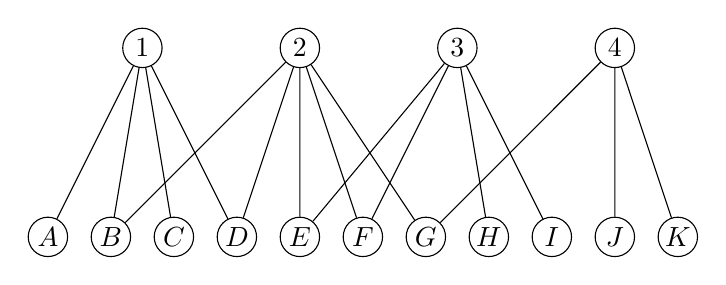
\begin{tikzpicture}[yscale=1.2,xscale=0.8]
      \node (1) at (1.5,1) {$1$};
      \node (2) at (4,1) {$2$};
      \node (3) at (6.5,1) {$3$};
      \node (4) at (9,1) {$4$};
      \node (A) at (0,-1) {$A$};
      \node (B) at (1,-1) {$B$};
      \node (C) at (2,-1) {$C$};
      \node (D) at (3,-1) {$D$};
      \node (E) at (4,-1) {$E$};
      \node (F) at (5,-1) {$F$};
      \node (G) at (6,-1) {$G$};
      \node (H) at (7,-1) {$H$};
      \node (I) at (8,-1) {$I$};
      \node (J) at (9,-1) {$J$};
      \node (K) at (10,-1) {$K$};

\foreach \b in {A,B,C,D}
  \draw (1) -- (\b);
\foreach \b in {B,D,E,F,G}
  \draw (2) -- (\b);
\foreach \b in {E,F,H,I}
  \draw (3) -- (\b);
\foreach \b in {G,J,K}
  \draw (4) -- (\b);
    \end{tikzpicture}
\end{document}
